\documentclass[a4paper,14pt]{extreport} % Розмір паперу А4, шрифт 14 пунктів
\usepackage[T2A]{fontenc}
\usepackage[english,ukrainian]{babel}
\usepackage{ucs}
\usepackage[utf8]{inputenc} % включємо кодування utf8 в *NIX (cp1251 в Windows)
\usepackage{amssymb,amsfonts,amsmath,mathtext,enumerate,float} % підключаємо пакети розширень
\usepackage{listings} % для вихідних кодів
\usepackage{alltt}  
\usepackage{algorithmic}
\usepackage{indentfirst} % для абзаців
\usepackage[pdftex]{graphicx}
\usepackage{titlesec}

\renewcommand{\rmdefault}{cmr}
\renewcommand{\sfdefault}{ftx}
\renewcommand{\ttdefault}{cmtt}

\makeatletter
\nocite{*}
\bibliographystyle{unsrt} % встановлюємо тип бібліографії

\renewcommand{\@biblabel}[1]{#1.} % змінюємо формат нумерації бібліографії на "цифра."
\makeatother

\usepackage{geometry} % Змінюємо поля сторінки
\geometry{left=3cm}
\geometry{right=1cm}
\geometry{top=2cm}
\geometry{bottom=2cm}

\usepackage{setspace} % інтерліньяж
\onehalfspacing

\addto\captionsukrainian{
  \renewcommand{\contentsname}{зміст}
  \renewcommand{\bibname}{перелік джерел}
}

\titleformat{\chapter}[display]
  {\normalfont\centering\Large\bfseries}
  {\chaptertitlename\ \thechapter}{0pt}{\Large\textsc}

% Змінюємо скрізь перелічення на наступні "цифра.цифра.":
\renewcommand{\theenumi}{\arabic{enumi}.} 	
\renewcommand{\labelenumi}{\arabic{enumi}.} 
\renewcommand{\theenumii}{.\arabic{enumii}.} 
\renewcommand{\labelenumii}{\arabic{enumi}.\arabic{enumii}.} 
\renewcommand{\theenumiii}{.\arabic{enumiii}.} 
\renewcommand{\labelenumiii}{\arabic{enumi}.\arabic{enumii}.\arabic{enumiii}.}

\righthyphenmin=2 % мінімальна к-ть символів для переносу
\sloppy

\begin{document}

	\newcommand{\signature}{
{\footnotesize
\begin{tabular}{@{}p{1in}@{}}
    \hrulefill \\
    \vspace{-\baselineskip}
    \centering{(підпис)}
\end{tabular}}
}

\newpage
\begin{titlepage}
\begin{center}
\textbf{КИЇВСЬКИЙ НАЦІОНАЛЬНИЙ УНІВЕРСИТЕТ ІМЕНІ ТАРАСА ШЕВЧЕНКА}\\
Факультет комп’ютерних наук та кібернетики\\
Кафедра теоретичної кібернетики
\end{center}
\vspace{1em}
\begin{center}
\Large{\textbf{Кваліфікаційна робота}}\\
\normalsize{\textbf{На здобуття ступеня бакалавра}}\\
за спеціальністю 122 Комп’ютерні науки

\vspace{0.5em}
на тему:

\large{\textsc{\textbf{Гомоморфне шифрування для захисту даних в хмарних та туманних технологіях}}}
\end{center}
\vspace{1em}
\begin{flushleft}
Виконав студент 4-го курсу\\
Дмитро МАЛЬОВАНИЙ
\hspace{\fill}\signature\\
\vspace{0.5em}
Науковий керівник:\\
професор, доктор фіз-мат. наук\\
Анатолій ПАШКО
\hspace{\fill}\signature\\
\end{flushleft}

\begin{flushleft}
    \hspace{18em}Засвідчую, що в цій роботі немає\\
    \hspace{15em}запозичень праць інших авторів без\\
    \hspace{15em}відповідних посилань.\\
    \vspace{0.3em}
    \hspace{15em}Студент\hspace{\fill}\signature\\
    \vspace{1em}
    \hspace{15em}Роботу розглянуто й допущено до захисту\\
    \hspace{15em}на засіданні кафедри\\
    \hspace{15em}теоретичної кібернетики\\
    \hspace{15em}"\vtop{\hsize=2em \hrulefill}"\vtop{\hsize=5em \hrulefill} 2023p\\
    \hspace{15em}протокол \No \vtop{\hsize=2em \hrulefill}\\
    \hspace{15em}Завідувач кафедри\\
    \hspace{15em}Юрій КРАК\hspace{\fill}\signature\\
\end{flushleft}

\vspace{\fill}

\begin{center}
Київ - 2023
\end{center}				
\end{titlepage}
 		% Титулка
 	\newpage
\chapter*{реферат}
Обсяг роботи 53 сторінки, 8 зображень, 5 лістингів, 33 джерел посилань.
ШИФРУВАННЯ, ГОМОМОРФНЕ ШИФРУВАННЯ, ХМАРНІ ТА ТУМАННІ КОМУНІКАЦІЇ, БЕЗПЕКА ПЕРЕДАЧІ ДАНИХ,
ЗАХИСТ ДАНИХ, БЕЗПЕКА, БЕЗПЕКА ДАНИХ В БАНКІВСЬКІЙ СИСТЕМІ.

Об'єктом роботи є дослідження можливостей використання гомоморфного шифрування в хмарних
та туманних обчисленнях. Предметом роботи, є реалізація спрощеної банківської системи, для
демонстрації можливостей гомоморфного шифрування.

Метою роботи є дослідження технології повного гомоморфного шифрування в хмарних та 
туманних технологій.

Методи розроблення: дослідження гомоморфних схем, аналітичне дослідження алгоритмів над
схемою. Інструменти розроблення: Мова С++, Бібліотека HeLib з вільно поширюваною ліцензією
Apache 2.0, додаткові бібліотеки для зручної роботи з Json, обробки та ініціації TCP 
з'єднань, та інш. 

Результати роботи: Описана логіка криптографічних схем гомоморфного шифрування, проведений
аналітичний огляд існуючих реалізацій схем, наведені переваги та недоліки використання 
технології гомоморфного шифрування, реалізований та продемонстрований в роботі застосунок
спрощеної банківської системи з використанням FHE.

Технологія гомоморфного шифрування, може використовуватись в будь-якій сфері де потрібна
конфіденційність даних, зокрема вона дозволяє тримати їх приватними для сторони яка їх
обробляє, що забезпечує ще вищий рівень безпеки.
		% Реферат
 	\newpage
\tableofcontents
 	% Зміст
    \newpage
\chapter*{скорочення та умовні позначення}
\addcontentsline{toc}{chapter}{\textsc{скорочення та умовні позначення}}

\textbf{\textsc{FHE}} -- Fully homomorphic encryption (Повне гомоморфне шифрування).

\textbf{\textsc{SHE}} -- Somewhat homomorphic encryption scheme

\textbf{\textsc{RSA}} -- Криптографічний алгоритм з відкритим ключем, який базується,
розрахунковій складності великих полупростих чисел.

\textbf{\textsc{PKI}} -- Public key infrastructure - набір інструментів які
використовують пару (приватний, публічний) ключ, та в якій між користувачами
передається тільки публічні ключі, залишаючи приватні анонімними.

\textbf{\textsc{Boolean Circuit}} -- Булева схема - це математична модель, що
використовується для представлення та обробки булевих функцій. Вона складається з логічних
елементів, які з'єднані між собою для виконання логічних операцій над двійковими входами
\(\{0,1\}\) та формування двійкових виходів. Схема складається з взаємопов'язаних логічних
елементів, таких як (AND, NOT, OR). 


\textbf{\textsc{FLT}} -- Мала теорема ферма \cite{Fermat}.
          % Скорочення та умовні позначення
 	
 	\newpage
\addcontentsline{toc}{chapter}{\textsc{вступ}}
\chapter*{\textsc{вступ}}


FHE або повне гомоморфне шифрування, це тип шифрування яке дозволяє виконувати розрахунки
на зашифрованих даних, не вимагаючи, щоб вони були розшифровані для цього. Результатом
розрахунків або ж гомоморфної операції над даними є зашифровані дані, які можуть бути
розшифровані ключем з тої ж самої пари, з якої вони були зашифровані.

Завдяки особливості виконувати операції над зашифрованими даними без попереднього
дешифрування, FHE стає гарним рішенням в задачах передачі даних в незахищених
середовищах, в не авторизованих середовищах, або при передачі над чутливих даних, які
не повинні бути видимі для сторони яка займається їх обробкою.

\subsection*{Оцінка сучасного стану об’єкта дослідження або розробки}
Вперше технологія FHE була запропонована в 1978 в році, але майже 30 років не було
авторитетних досліджень на цю тему і на той момент вже існувала система RSA, яка була
краща за багатьма параметрам. Починаючи з 2009 року дослідження та розробки на
тему гомоморфного шифрування дуже актуальні й розвиток цієї технології відбувається
надзвичайно швидко, покращуючи швидкість виконання операцій, швидкість дешифрування, та
розширюючи область застосування шляхом додавання більш комплексних гомоморфних операцій.
На цей час існує багато рішень на типові проблеми з використовуванням FHE, які
конкурують між собою в різних аспектах, та постійно розвиваються.

\subsection*{Актуальність роботи та підстави для її виконання}
Безпечність передачі даних в незахищених середовищах та авторизація отримувача були 
завжди дуже важливими, рідко хто нехтує цим, оскільки не хоче, щоб їх данні були
скомпрометовані або перехоплені. Окрім цього все частіше, за потребою складних
обчислень, користувачі звертаються до віддалених машин, також відомі як хмари. Звісно
кожен користувач хоче, щоб їх данні були захищенні під час передачі, та хоче бути
впевнений, що він передає данні саме туди, куди планував.

Для забезпечення вище описаних вимог, користувач використовує чинні технології, такі
як PKI. Єдина не вирішена проблема PKI або інших технологій, це вимога повного
дешифрування даних, це означає що при отриманні зловмисником доступу до хмари або
віддаленого сервера, у нього буде доступ до не зашифрованих даних. Хоча сучасні хмари
дуже добре захищенні, розраховувати на те що зловмисник не зможе отримати до них
доступ - не варто. 

Для розв'язання проблеми, яку не вирішує PKI, чудово підходить FHE, оскільки сервер,
зберігає і виконує операції над даними в зашифрованому вигляді, тому навіть якщо
зловмисник отримає доступ до сервера або хмари, отримати дані в нього не вдасться.

Звісно є і деякі обмеження у використанні FHE: по-перше, операції над даними
обов'язково повинні бути гомоморфні, по-друге, алгоритм застосування операції над
зашифрованими даними дуже повільний. Якщо задача вимагає обробку великої кількості
даних, або операція повинна бути не гомоморфна, то можливо краще подумати в сторону
застосування інших криптосистем.

\subsection*{Мета й завдання роботи}
Написати пізніше
\subsection*{Об’єкт і методи дослідження}
об’єкт і методи дослідження або розроблення

\subsection*{Можливі сфери застосування}
Гомоморфне шифрування може бути застосоване в будь-якій сфері де потрібна обробка
даних, та для виконання цієї задачі використовується віддалений сервер, або хмара.
Використання FHE, гарантує безпечну передачу та обробку без попереднього дешифрування
даних, але при цьому накладає обмеження на операцію обробки, яка повинна бути
гомоморфна, та значно знижує час обробки.
 			% Вступ
 
 	\newpage

\chapter{\textsc{огляд технології FHE}}


\section{Визначення}
В цій секції описана термінологія, яка використовується в дослідженнях FHE. Деякі з 
визначень були взяті напряму з документів FHE, інші були перефразовані для того, щоб
спростити формальність і зробити їх більш застосованими до обраної задачі.

Нехай є простір вхідного (чистого) тексту \(\mathcal{P}=\{0,1\}\), та сімейства функцій
\(F={f_1,f_2,...,f_n}\) де \(f_n(x) = f(x_1,x_2,x_3,...,x_k)\) це Булеві функції k
аргументів: \(f: P^n \rightarrow P\). Ми будемо називати F, сімейством Булевих схем
(Boolean circuit) \(C\), і використовувати звичайний запис функції \(C(m_1,m_2,...,m_n)\),
для позначення оцінки Булевої схеми на кортежі \((m_1,m_2,...,m_n)\).

\begin{definition}[\(\mathcal{C}\)-схема розрахунків, або ж просто \(\mathcal{C}\)-схема \cite{cryptoeprint:2011/344}] 
    Нехай \(\mathcal{C}\) це множина Булевих схем, тоді \(\mathcal{C}\)-схема розрахунків, для
    \(\mathcal{C}\) це набір функцій \((\textsc{gen, enc, eval, dec})\) які задовільняють наступним твердженням:


\(\textsc{\textbf{gen}}(1^\lambda,\alpha)\) - алгоритм генерації ключів, на вхід він приймає,
параметр шифрування \(\lambda\), та допоміжний параметр \(\alpha\). Результат виконання
алгоритму це триплет ключів \((pk,sk,evk)\), де ключ \(pk\) використовується для шифрування,
\(sk\) для дешифрування, та  \(evk\) для виконування розрахунків.

\(\textsc{\textbf{enc}}(pk,m)\) - алгоритм шифрування, на вхід він приймає ключ шифрування \(pk\) та
фрагмент не зашифрованого (чистого) тексту \(m\). Результат виконання алгоритму це шифр \(c\).

\(\textsc{\textbf{eval}}(evk,C,c_1,c_2...,c_n)\) - алгоритм розрахунків. На вхід він отримує,
ключ розрахунків \(evl\) та Булеву схему \(C \in \mathcal{C}\), та вхідні аргументи, які
можуть бути як шифром, так і результатом виконання минулих розрахунків. Результат виконання
алгоритму це результат виконання розрахунків.

\(\textsc{\textbf{dec}}(sk, c)\) - алгоритм дешифрування. На вхід приймає, ключ дешифрування
\(sk\), та шифр, або результат виконання розрахунків. Результат виконання алгоритму це не
зашифрований (чистий) текст \(m\).
\end{definition}

Для подальшого опису властивостей, треба визначити простори даних, які є результатами, або
вхідними параметрами описаних алгоритмів:

Нехай \(\mathcal{X}\) буде описувати простір \emph{чистого шифру}, \(\mathcal{Y}\) -
простір результатів виконання розрахунків, і \(\mathcal{Z} = \mathcal{X} \cup \mathcal{Y}\).
\(\mathcal{Z^*}\) - містить кортежі довільної довжини, які складаються
з елементів \(\mathcal{Z}\). Простори ключів згенерованих \textsc{\textbf{gen}},
позначимо як \(\mathcal{K}_p,\mathcal{K}_s,\mathcal{K}_e\) для \(pk,sk,evk\) відповідно.Алгоритм \textsc{\textbf{gen}} приймає на вхід параметр в унарній нотації \(1^\lambda\)
та опціональний допоміжний параметр \(\lambda\) з простору \(\mathcal{A}\). Також,
\(\mathcal{C}\) містить простір \emph{дозволених} булевих схем, а \(\mathcal{P}\), як було
зазначено раніше, область вхідного \emph{чистого (незашифрованого)тексту}.

Тепер можна описати область роботи наведених вище алгоритмів:
\begin{center}
    \begin{tabular}{l}
        \textsc{\textbf{gen }}: 
        \begin{math}
            \mathbb{N}\ \times\ \mathcal{A}\ \rightarrow\ 
            \mathcal{K}_p\ \times\ \mathcal{K}_s\ \times \ \mathcal{K}_e
        \end{math}\\

        \textsc{\textbf{enc }}:
        \begin{math}
            \mathcal{K}_p\ \times\ \mathcal{P}\ \rightarrow\ \mathcal{X}
        \end{math}\\

        \textsc{\textbf{eval}}:
        \begin{math}
            \mathcal{K}_e\ \times\ \mathcal{C}\ \times\ \mathcal{Z}^*\ 
            \rightarrow\ \mathcal{Y}
        \end{math}\\

        \textsc{\textbf{dec }}:
        \begin{math}
            \mathcal{K}_s\ \times\ \mathcal{Z}\ \rightarrow\ \mathcal{P}
        \end{math}
    \end{tabular}
\end{center}

Тоді \(\mathcal{X}\) та \(\mathcal{Y}\) можна визначити наступним чином:
\begin{center}
    \begin{math}
        \mathcal{X}\ =\ \{c\ |\ \textsc{\textbf{enc}}(pk,m)\ =\ c,\ m\ \in\ \mathcal{P}\}
    \end{math}
    \begin{math}
        \mathcal{Y}\ =\ \{z\ |\ \textsc{\textbf{eval}}(evk,C,c_1,c_2,...,c_n) = z,\ c_i\ \in\ 
        \mathcal{Z},\ C\ \in\ \mathcal{C} \}
    \end{math}
\end{center}
В деяких схемах, ключі розрахунків та шифрування однакові, але часто це і не так, тому в
визначеннях було наведено більш спільний випадок.

В оригінальних документах FHE \cite{cryptoeprint:2011/344} не було зазначено, що алгоритм
розшифровування \textsc{\textbf{dec}} повинен мати можливість працювати з результатом виконання
алгоритму шифрування \textsc{\textbf{enc}} - \(\mathcal{X}\), і було зазначено, що данні
можуть бути розшифровані після виконання розрахунків над ними \textsc{\textbf{eval}} - 
\(\mathcal{Y}\). Для можливості розшифровування, зразу після зашифровування було запропоновано
мати \emph{чисту Булеву схему} або ж по суті функцію \(f(x)=x\), для виконання розрахунків і
отримання даних які вже можна буде розшифровувати. Більшість сучасних FHE схем, дозволяють
проводити операції дешифрування даних, над якими не було проведено розрахунків, тому я не буду
заглиблюватись в цю тему.

\subsection{Атрибути та властивості}
Тут представлені характеристики методів гомоморфного шифрування. Ми встановлюємо такі
властивості, як компактність і конфіденційність схеми, які забороняють спрощені рішення
задачі гомоморфного шифрування, з одного боку, і вимагають таких властивостей, як
коректність, для того, щоб навіть називати це схемою шифрування.

\begin{definition}[Коректне розшифровування \cite{cryptoeprint:2015/1192}]
\label{def:corr-dec}
\(\mathcal{C}\)-схама має атрибут коректного розшифрування якщо виконується наступне твердження:
\begin{center}    
    \begin{math}
        \textsc{\textbf{dec}}(sk,\textsc{\textbf{enc}}(pk,m)) = m
    \end{math},\\
    де \(pk,sk,evk \leftarrow \textsc{\textbf{gen}}(1^\lambda,\alpha)\), \(\alpha \in \mathcal{A}\), \(m \in \mathcal{P}\).
\end{center}
Це означає, що ми повинні мати можливість безпомилково розшифровувати зашифрований текст.
\end{definition}

\begin{definition}[Коректні розрахунки \cite{cryptoeprint:2015/1192}]
\label{def:corr-eval}
\(\mathcal{C}\)-схема коректно розраховує всі Булеві схеми \(C \in \mathcal{C}\), якщо
виконується наступне твердження:
    \begin{center}
        \begin{math}
        \textsc{\textbf{dec}}(sk,\textsc{\textbf{eval}}(evk,C,c_1,c_2,...,c_n))\ 
        =\ C(m_1,m_2,...m_n)
        \end{math},\\
        \(pk,sk,evk \leftarrow \textsc{\textbf{gen}}(1^\lambda,\alpha)\), \(\alpha \in \mathcal{A}\), \(c_i \in \mathcal{X}\) та \(m_i \leftarrow \textsc{\textbf{dec}}(sk,c_i)\)
    \end{center}
Це визначення означає, що розрахунки над зашифрованими даними з подальшим
розшифровуванням повинні бути однакові з результатом розрахунків над не зашифрованими
даними.
\end{definition}

Будемо називати \(\mathcal{C}\)-схему \emph{коректною} якщо для неї будуть виконуватись
\ref{def:corr-dec} та \ref{def:corr-eval} твердження.

\begin{definition}[Компактність \(\mathcal{C}\)-схеми]
\label{def:compactness}
    \(\mathcal{C}\)-схема вважається компактною якщо існує поліном \(p\), такий що, для
    будь-якого кортежу \((pk,sk,evk) \leftarrow \textsc{\textbf{gen}}(1^\lambda,\alpha)\), \(\alpha \in \mathcal{A}\), будь-якої Булевої схеми \(C \in \mathcal{C}\) та
    шифру \(c_i \in \mathcal{X}\), розмір результату виконання
    \(\textsc{\textbf{eval}}(evk,C,c_1,c_2,...,c_n)\) не більше від \(p(\lambda)\)
    бітів, в не залежності від Булевої схеми.
\end{definition}
Визначення \ref{def:compactness}, показує що під час гомоморфних операцій розмір
результату не повинен збільшуватись, і залежить тільки від параметра безпеки \(\lambda\).

\begin{definition}[Компактно розрахункова \(\mathcal{C}\)-схема \cite{homenc}]
\label{def:compactl-eval}
\(\mathcal{C}\)-схема компактно розраховує всі Булеві схема \(C \in \mathcal{C}\), якщо
вона компактна \ref{def:compactness} та \emph{коректна}.
\end{definition}

\subsubsection*{Безпека схеми}
Далі, важливо зупинитись на безпеці та конфіденційності схеми. Безпеку схеми можна
розділити на дві компоненти: семантична безпека, та обфускація схеми. Якщо обфускація
використовується коли алгоритм шифрування секретний, і вразливий, то семантична безпека
описує розподіл вихідних даних з \textsc{\textbf{eval}} та \textsc{\textbf{enc}}.
\begin{definition}[Приватне гомоморфне шифрування схеми \cite{homenc}(2.16)]
    \(\mathcal{C}\)-схема вважається безпечною, якщо для будь-якого кортежу \((pk,sk,evk) \leftarrow \textsc{\textbf{gen}}(1^\lambda,\alpha)\), \(\alpha \in \mathcal{A}\), будь-якої Булевої схеми \(C \in \mathcal{C}\) та
    шифру \(c_i \in \mathcal{X}\), такого що \(m_i \leftarrow \textsc{\textbf{dec}}(sk, c_i)\) існує два розподіли:

\begin{center}
    \begin{math}
        Dist_1 = \textsc{\textbf{eval}}(evk,C,c_1,c_2,...,c_n)
    \end{math}\\
    \begin{math}
        Dist_2 = \textsc{\textbf{enc}}(pk,C(c_1,c_2,...,c_n)
    \end{math}
\end{center}
які повинні бути статистично або обчислювально нерозрізнені. Ці вимоги показують,
що розподіл виконання обчислень Булевої схеми над шифром \(Dist_1\) повинен бути однаковий (статистично, обчислювально) з розподілом, отриманим шляхом зашифровування
\emph{чистого} тексту, який насамперед являється результатом виконання Булевої операції 
над незашифрованими даними \(Dist_2\).

Часто термін безпечної системи можна зустріти як \emph{Сильно гомоморфна система}\cite{Clear_2013}. 
\end{definition}

\subsection{Класифікація}
Оскільки не всі схеми FHE мають однакові властивості, цей розділ показує як схеми
класифікуються, в залежності від того, які схеми вони можуть обчислювати.

\begin{definition}[Частково Гомоморфна схема або \(\mathcal{C}\)-Гомоморфізм \cite{cryptoeprint:2011/344}]
\(\mathcal{C}\)-схема називається, частково гомоморфною (SHE), якщо вона має коректне
шифрування \ref{def:corr-dec}, та коректне обчислення \ref{def:corr-eval}.
\end{definition}
Для частково гомоморфних \(\mathcal{C}\)-схем нема вимог до компактності, тому з кожним
гомоморфним розрахунком розмір вихідного шифру може збільшуватись. Також нема ніяких
вимог до множини Булевих операцій які можуть бути використовувані для розрахунків.

\begin{definition}[Обмежено-рівнева Гомоморфна схема]
\(\mathcal{C}\)-схема називається Обмежено-рівневою, якщо алгоритм генерації ключів
\textsc{\textbf{gen}} приймає додатковий параметр \(\alpha=d\), який означає максимальну
глибину Булевої схеми, яка може бути обчислена. Також застосовані вимоги до компактності,
коректності, і те що розмір вихідних даних розрахунків не повинен залежати від d.

\end{definition}

\begin{definition}[Повна Гомоморфна схема]
Повною гомоморфною схемою, називають \(\mathcal{C}\)-схему, до якої застосовані вимоги,
коректності, компактності, та вона може обчислювати Булеву схему з множини усіх схем, або
ж будь-яку схему.
\end{definition}

\subsection{Композиція розрахунків}
Часто, задача потребує декілька послідовних розрахунків, тобто результат певної Булевої
схеми повинен слугувати вхідними даними для наступної схеми, або ж простими словами
можна це назвати - композиція.
Кожну операцію розрахунків над шифром \textsc{\textbf{eval}} будемо називати \emph{етапом розрахунків}. 

З визначення коректних розрахунків \ref{def:corr-eval} видно що вхідні дані для
алгоритму обчислення \textsc{\textbf{eval}} повинні належати множині \(\mathcal{X}\) -
або ж множині \emph{чистого шифру}, який є результатом алгоритму \textsc{\textbf{enc}}.
Цей розділ описує вимоги, виконуючи які алгоритм розрахунку схеми \textsc{\textbf{eval}},
може приймати на вхід як результат виконання інших розрахунків \(\mathcal{Z}\), так і
\emph{чистий шифр} \(\mathcal{X}\): 

\(\textsc{\textbf{eval}}(evk, C, c_1,c_2,...,c_n)\),
де \((pk,sk,evk) \leftarrow \textsc{\textbf{gen}}(1^\lambda,\alpha)\), \(\alpha \in \mathcal{A}\), \(C \in \mathcal{C}\) та \(c_i \in \mathcal{X} \cup \mathcal{Z}\)

В літературі \emph{розрахунки з етапами} називають \textbf{\emph{гомоморфним шифруванням
з i-стрибками}}(i-hop homomorphic encryption \cite{10.1007/978-3-642-19571-6_14},
\cite{cryptoeprint:2010/145})

\begin{definition}[Розрахунки з етапами]

\end{definition}

\section{Обмеження}


\section{Відомі області застосування}
  		% Розділ 1
% 	\newpage

\chapter{\textsc{Використання FHE в хмарних технологіях}}

\section{Бібліотека HeLib}
Для реалізації поставленої задачі буде використовуватись бібліотека гомоморфного шифрування
HeLib. HeLib була написана на С++ та реалізовує функціонал  Brakerski-Gentry-Vaikuntanathan 
(BGV), та Cheon-Kim-Kim-Song (CKKS) схем.

З середини 2018 року HElib знаходиться на стадії інтенсивного рефакторінгу для підвищення
надійності, розширяємості, продуктивності та, найголовніше, легкості у використанні для дослідників та розробників, які працюють з HE та його застосуванням.

Нижче представлені деякі ключові аспекти того, як HElib реалізує схему FHE:
\begin{itemize}
\item{\textsc{\textbf{Шифрування на основі поліномів}}: HElib використовує схему
    шифрування на основі поліномів, де відкриті текстові повідомлення 
    (\emph{чистий текст}) подаються у вигляді поліномів над скінченним полем. 
    Процес шифрування полягає у перетворенні текстового повідомлення у поліном, а потім у
    застосуванні до нього деяких математичних операцій.}

\item{\textsc{\textbf{Генерація ключів}}: HElib генерує набір ключів, необхідних для
    шифрування, розшифрування та гомоморфних операцій. Ці ключі включають секретний ключ,
    відкритий ключ та розрахункові ключі. Секретний ключ зберігається у таємниці, тоді як
    відкритий ключ надається стороні, яка виконує обчислення. Розрахункові ключі
    використовуються для виконання гомоморфних операцій над зашифрованими даними.} 

\item{\textsc{\textbf{Шифрування}}: Щоб зашифрувати відкрите повідомлення, HElib перетворює
    його у поліном і застосовує операції шифрування з використанням відкритого ключа. Цей
    процес включає додавання шумового члена до полінома для забезпечення безпеки.}

\item{\textsc{\textbf{Гомоморфні операції}}: HElib підтримує різні гомоморфні операції,
    такі як додавання, множення та обертання. Ці операції дозволяють виконувати обчислення
    над зашифрованими даними без їх розшифрування. Для виконання цих операцій HElib
    використовує математичні методи, такі як поліноміальне множення та модулярна арифметика.}

\item{\textsc{\textbf{Розшифрування}}: Щоб розшифрувати результат обчислень, HElib
    використовує секретний ключ і застосовує операції дешифрування. Шумовий член, доданий
    під час шифрування, зменшується під час розшифрування, щоб отримати вихідне
    повідомлення у відкритому вигляді.}

\item{\textsc{\textbf{Оптимізація продуктивності}}: HElib включає декілька оптимізацій
    продуктивності для підвищення ефективності обчислень FHE. Ці оптимізації включають такі
    методи, як перемикання модулів, завантаження та пакування декількох значень відкритого
    тексту в один зашифрований текст.}
\end{itemize}

\subsection{Алгоритми над схемою}
\begin{itemize}
\item{\textsc{\textbf{Гомоморфне додавання:}}
    Гомоморфне додавання дозволяє додавати два поліноми зашифрованого тексту, в результаті
    чого виходить новий поліном зашифрованого тексту, що представляє собою суму відповідних
    поліномів відкритого тексту.

    Процес гомоморфного додавання полягає у додаванні коефіцієнтів поліномів зашифрованого
    тексту за модулем скінченного поля. Математично, для двох поліномів шифрованого тексту
    \(C_1(x)\) і \(C_2(x)\), що представляють поліноми відкритого тексту \(P_1(x)\) і 
    \(P_2(x)\) відповідно:
    \begin{math}
        C_1(x) + C_2(x) = (P_1(x) + P_2(x))\ mod\ q
    \end{math}, де \(q\) - модуль скінченного поля.

    Оскільки додавання є простою операцією, то додавання поліномів зашифрованого тексту
    можна виконувати безпосередньо, член за членом, без необхідності розшифровувати
    поліноми. Ця властивість дозволяє проводити обчислення над зашифрованими даними без
    розкриття оригінального відкритого тексту.
}
\item{\textsc{\textbf{Гомоморфне множення:}}
    Гомоморфне множення дозволяє перемножити два поліноми зашифрованого тексту, в
    результаті чого новий поліном зашифрованого тексту є добутком відповідних поліномів
    відкритого тексту.

    Процес гомоморфного множення є більш складним і вимагає додаткових кроків:
    \begin{enumerate}
        \item{\textbf{Перемноження}:
            Для множення двох поліномів зашифрованого тексту виконується операція множення
            поліномів. Ця операція передбачає множення коефіцієнтів поліномів разом, член
            за членом. Результуючий поліном являє собою поточковий добуток поліномів
        відкритого тексту.}
        \item{\textbf{Зведення до спільного степеню за модулем}:
            Після множення многочленів, результуючий многочлен може мати більш високі
            степені через процес множення. Щоб зберегти цілісність схеми шифрування,
            отриманий поліном потрібно зменшити по модулю на певний коефіцієнт. Цей множник
            часто пов'язаний з модулем q скінченного поля.}
        \item{\textbf{Обмін ключами}: 
            Для продовження виконання гомоморфних операцій над отриманим поліномом
            застосовується процес, який називається \emph{обмін ключів}. Обмін ключів
            дозволяє перетворити ключ шифрування, який використовувався під час шифрування,
        на ключ розрахунків, що дає змогу продовжити гомоморфні обчислення.}
    \end{enumerate}
}
\item{\textsc{\textbf{Гомоморфне обертання:}}
    Гомоморфне обертання дозволяє зміщувати коефіцієнти полінома зашифрованого тексту, тим
    самим змінюючи порядок даних у поліноміальному поданні. Ця операція особливо корисна
    для виконання операцій над підмножинами даних або перестановки полінома відповідно до
    бажаних обчислень.

    Для досягнення гомоморфного обертання можна використовувати різні методи, такі як
    операції модулярної арифметики, матриці перестановок або інші специфічні для шифрування
    методи. Ці методи дозволяють ефективно зміщувати коефіцієнти, зберігаючи при цьому
    властивості шифрування.
}

\end{itemize}
Важливо відзначити, що гомоморфні операції вносять шум і можуть впливати на безпеку і
точність обчислень. У міру виконання операцій шумовий член накопичується і може вимагати
додаткових кроків, наприклад застосування описаної раніше техніки повторного шифрування,
щоб зберегти безпеку і правильність обчислень.

Використовуючи гомоморфне додавання, множення і обертання, обчислення можна виконувати над
зашифрованими даними без їх розшифровки, що дозволяє проводити обчислення з дотриманням
конфіденційності, зберігаючи при цьому конфіденційність відкритих текстових
повідомлень.

\section{Реалізація застосунку}
Для демонстрації коректності роботи, та можливості застосування FHE схеми у хмарних 
технологіях, був реалізований клієнт-серверний застосунок. Застосунок повинен реалізовувати
логіку банківської системи, тобто клієнт повинен мати можливість створити рахунок,
додати баланс, та зняти баланс з рахунку. Окрім цього, система бути розроблена з розрахунком
на те що вона буде знаходитись на хмарі, та між клієнтом і хмарою буде незахищене з'єднання.
Також, користувач банківського сервісу хоче бути впевнений в повному захисті даних, в тому
числі від сервера. Для реалізації вимог для безпеки даних буде використана FHE з реалізацією
BGV схеми в бібліотеці HeLib. Див. Рис 2.1.

\begin{figure}[!ht]
    \centering
    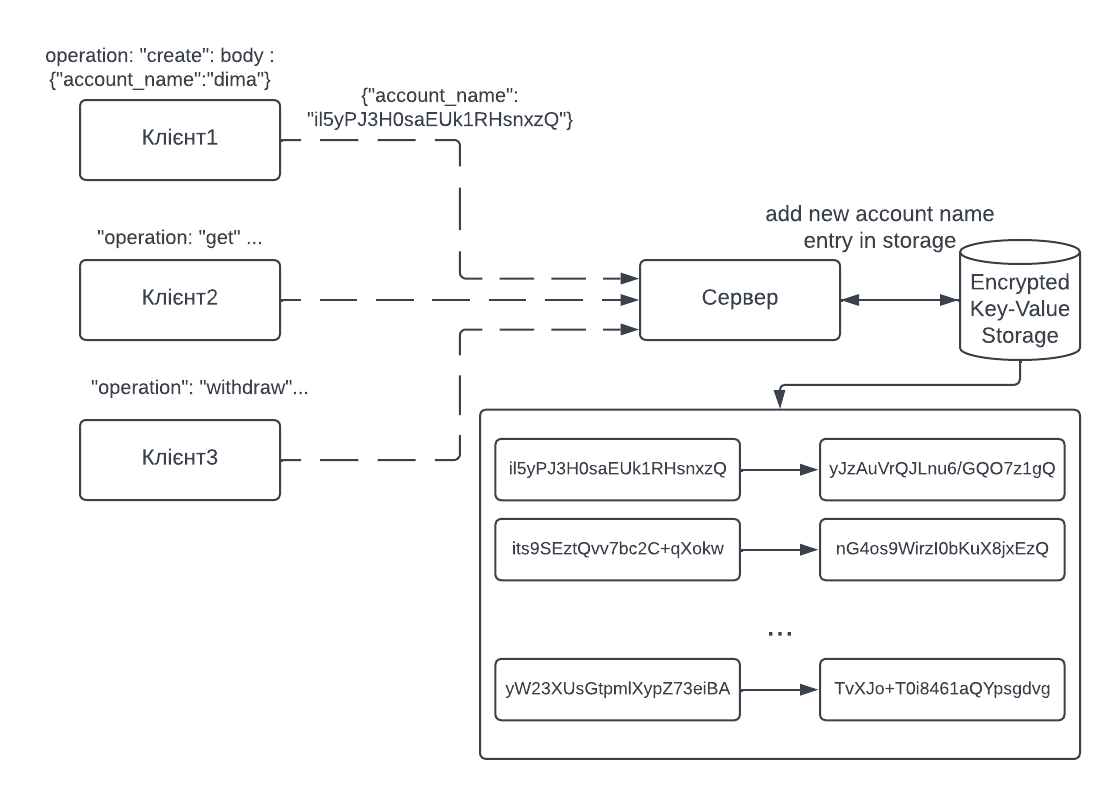
\includegraphics{static/client-server-logic.png}
    \caption{Демонстрація запитів клієнтів до серверу, де перервана стрілочка, означає
    незахищене середовище, тому данні в ньому будуть зашифровані}
    \label{fig:client-server-logic}
\end{figure}

\subsection{Вимоги}
Ця секція описує вимоги до розробки банківської системи, яка повинна забезпечувати коректність,
та безпеку даних.
\subsubsection*{Клієнт}
Основна задача клієнта, це створити необхідний контекст для FHE шифрування, ініціювати
з'єднання з сервером, робити необхідні запити, та обробляти відповіді від сервера.

Як було написано вище, клієнт повинен бути відповідальний за створення контексту шифрування. Під
контекстом, будемо вважати необхідні дані для правильного працювання FHE, зашифровування та розшифровування даних.
Деяку частину контекста необхідно буде надати серверу для того, щоб він мав можливість виконувати
розрахунки над зашифрованими даними, проте частина контекста повинна бути нерозголошуєма, така як
приватний ключ.

Контекст буде зберігатись на машині клієнта у файлі Json формату, і при ініціюванні з'єднання
з сервером, у клієнта повинна бути можливість вибору, чи створювати новий контекст, чи використати
присутній.

Нехай контекст був згенерований з деякими тестовими параметрами тоді його Json, та приватний
ключ буде виглядати наступним чином:

\begin{lstlisting}[breaklines, caption={Json репрезентація, контексу, деякі довгі послідовносиі чисел були замінені на трикрапку, щоб зменшити кількість тексту}, 
captionpos=b]
{"HElibVersion":"2.2.0","content":{"alsoThick":false,"build_cache":false,"digits":[[6,"..."],[11,"..."]],"ePrime_param":4,"e_param":12,"gens":[2341,3277,911],"hwt_param":120,"m":4095,"mvec":[7,"..."],"ords":[6,4,6],"p":2,"qs":[249047285761,"..."],"r":1,"scale":10.0,"smallPrimes":[0,"..."],"specialPrimes":[15,"..."],"stdev":{"exponent":0,"mantissa":3.2}},"serializationVersion":"0.0.1","type":"Context"}
\end{lstlisting}

\begin{lstlisting}[breaklines, caption={Json репрезентація приватного ключа}, captionpos=b]
{"HElibVersion":"2.2.0","content":{"b":[{"map":[[ large amount of 64-bits integers]],"set":[6,7,...]}]},"serializationVersion":"0.0.1","type":"SecKey"}
\end{lstlisting}
Клієнт повинен правильно серіалізувати свій контекст, для подальшого відправлення серверу,
та приватний ключ, для зберігання.

\begin{lstlisting}[breaklines, caption={Json формат зберігання приватного контексту на 
клієнті, для можливості його подальшого використання}, captionpos=b]
{
    "public_context": "Listing 2.1",
    "private_key": "Listing 2.2"
}
\end{lstlisting}

Для того щоб клієнт мав можливість перевикористовувати створений ним контекст, був
розроблений додатковий скрипт, який зберігає публічний та приватний контекст в файл.
Клієнт при ініціюванні з'єднання з сервером моє можливість вибрати файл з контекстами,
або ж використати новий (згенерований).

\subsubsection*{Сервер}
Задача серверної частини застосунку, це приймати TCP/IP з'єднання, та коректно обробляти 
запити від клієнта. Окрім глобальної задачі сервера, він повинен виконувати якусь логіку.

Також для зручного використання на хмарі, сервер повинен мати інструмент автоматичної розгортки,
для цього буде використана технологія контейнеризації Docker.

Фактично, логіку серверу можна поділити на 2 частини:
\begin{itemize}
    \item{\textbf{Пошук сутності в зашифрованій базі даних}: Хоча задача пошуку даних в базі
даних, може здатись тривіальною задачею, коли сервер працює повністю над зашифрованими даними,
задача стає дещо складнішою, оскільки шифрування одних і тих самих даних, може давати різний
результат кожен раз, тому просте зіставлення з даними в базі не дасть коректного результату.

Для коректного знаходження даних в базі, за ключем буде використовуватись наступний алгоритм:

Нехай у нас є сховище ключ-значення Рис. 2.2.


\begin{figure}[!ht]
    \centering
    \label{fig:key-value-storage}
    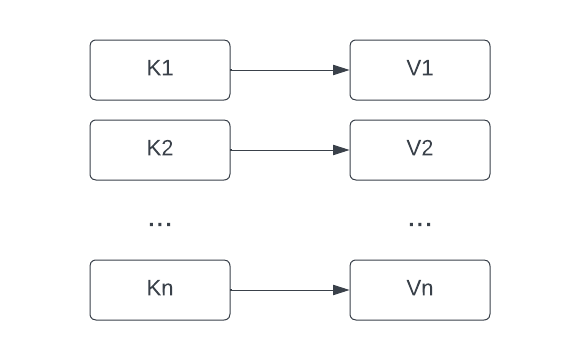
\includegraphics[scale=1.25]{static/key-value-storage.png}
    \caption{Де \(K\)- це множина ключів, та \(k_1,k_2,...,k_n \in K\), \(v_1, v_2,...,v_n 
    \in V\), де \(V\)- це множина значень, а \(n\)-кількість сутностей в базі. Тобто
    відображення \(K \rightarrow V\) є бієктивним.}
\end{figure}

    Високорівнево, алгоритм пошуку в базі, над зашифрованими даними описаний на заображенні
    Рис. 2.3.

\begin{figure}[!ht]
    \label{fig:basic-value-extraction}
    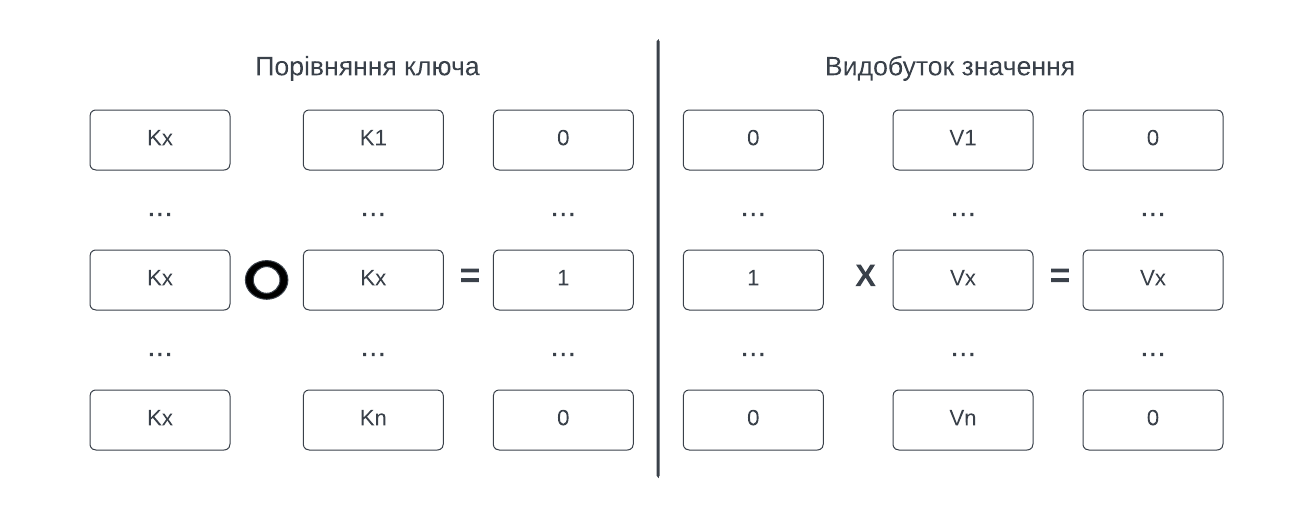
\includegraphics[scale=0.85]{static/basic-value-extraction.png} 
    \caption{Спрощений алгоритм пошука значення \(V_x \in V\), за ключем \(K_x \in K\)}
\end{figure}

    Далі буде описано більш детально алгоритм пошуку за ключем в зашифрованій базі даних.
    
    Першим кроком алгоритму є обчислення операції різниці між запитом і ключами бази даних. Це
    проста операція віднімання, яка поелементно виконує віднімання у структурі, схожій на масив. В
    результаті буде отримано різницевий шифротекст, який ми позначимо як \(\Delta_i\) де
\(\Delta_1,\Delta_2,...,\Delta_n \in \delta\). Наразі 
    \(\Delta = 0\) якщо \(k_q \in K\), і ненульовому значенню в іншому випадку, див. Рис. 2.4.

\begin{figure}[!ht]
    \centering
    \label{fig:key-subsruction}
    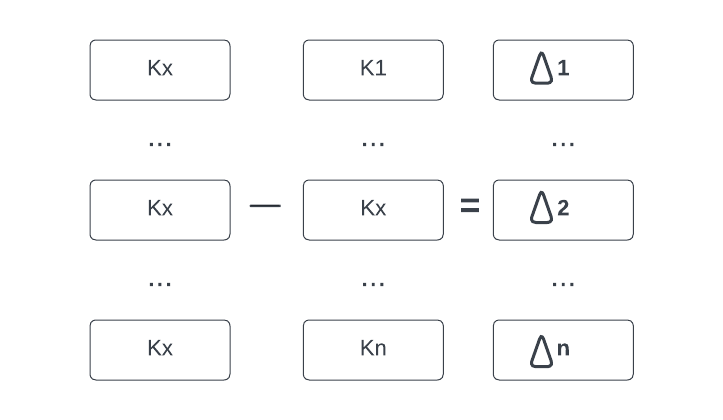
\includegraphics[scale=1.25]{static/key-substruction.png}
    \caption{Віднімання ключів, щоб отримати \(\Delta_1,\Delta_2,...,\Delta_n \in \delta\).
    Де у випадку \(K_q \in K\, \Delta_q = 0, \Delta_i \neq 0, i \neq q\)}.
\end{figure}


Це не зовсім та маска, яка нам потрібна, тому ми повинні виконати іншу операцію, описану далі.
Для отримання правильної маски, треба буде застосувати малу теорему Фермa  \cite{Fermat} до
\(\Delta_i \in \delta\). Застосувавши теорему, ми отримаємо наступний результат:

\begin{align*}
\text{LTF}(\Delta_i) =
\begin{cases} 
    1, & \Delta_i \neq 0 \\
    0, & \Delta_i = 0
\end{cases}
\end{align*}

Проте, ця маска дає обернений результат, щоб отримати коректні значення, треба застосувати
операцію інверсії:

\begin{align*}
1- \text{LTF}(\Delta_i) =
\begin{cases} 
    0, & \Delta_i \neq 0 \\
    1, & \Delta_i = 0
\end{cases}
\end{align*}

Якщо описати процес знаходження над зашифрованими даними \textsc{\textbf{enc}}(\(x\)), то це
буде виглядати так, як зображено на Рис. 2.5.

Спочатку ми застосовуємо операцію малої теореми Ферма (FLT) \cite{Fermat} до кожного різницевого
зашифрованого тексту. Це призводить до шифрування нуля, \(E(0)\), якщо різниця дорівнює нулю,
тобто є збіг, і шифрування одиниці, \(E(1)\), в іншому випадку.

Далі ми використовуємо попередньо обчислені результати операції FLT і віднімаємо це значення від
1. Це значення 1 може бути чистим, оскільки будь-яка операція між зашифрованим текстом і
відкритим текстом призводить до зашифрованого тексту. Це призводить до відображення будь-якого
ненульового значення в нуль і нуля в одиницю. Таким чином, ми отримуємо маски, які нам потрібні
для алгоритму порівняння. 

Однак є ще один аспект, який слід взяти до уваги, а саме: як ми повинні діяти з частковими збігами?

\begin{figure}[!ht]
    \centering
    \label{fig:mask-creation-flow}
    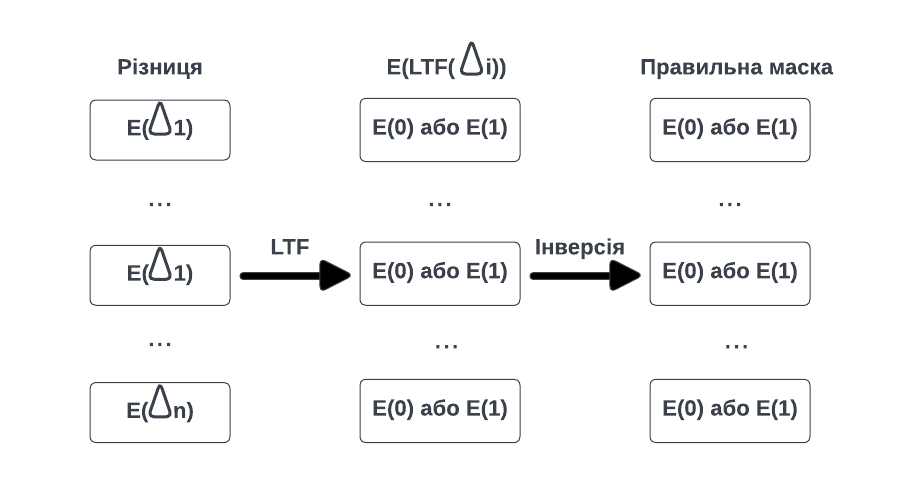
\includegraphics[scale=1.25]{static/mask-creation-flow.png}
    \caption{Процес створення правильної маски над зашифрованими даними}
\end{figure}
Розглянемо наступний сценарій, показаний на зображенні нижче Рис 2.6. Уявіть, що ключ збігається лише з
другою літерою запиту і, можливо, з деякими значеннями пропусків, тоді він створить масив, як
показано нижче Рис. 2.6.

Оскільки в нашому прикладі нас цікавлять лише точні збіги, цей результат слід вважати таким, що
не збігається. Щоб усунути часткові збіги, ми просто копіюємо зашифрований текст, виконуємо
обертання структури масиву в копії і перемножуємо його за входом з оригінальною копією. Це
означає, що якщо в одному з осередків зашифрованого тексту є хоча б один 0, то цей осередок
ефективно обнулить всі інші осередки масиву.

Зауважте, що оскільки ми не можемо знати, який саме шифротекст містить результат, що збігається,
частково збігається або не збігається, ця операція також виконується над результатом, що
збігається. Однак, оскільки у зашифрованому тексті у кожному слоті має бути 1, то ця операція не
повинна мати ніякого ефекту.

\begin{figure}[!ht]
    \centering
    \label{fig:partial-match}
    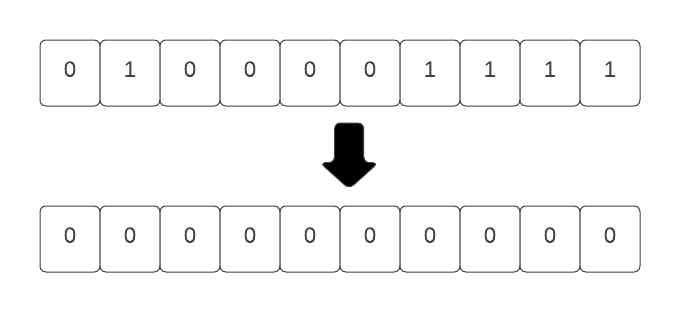
\includegraphics{static/partial-match.png}
    \caption{Частковий збіг, який не повинен вважатись коректним}
\end{figure}

Тепер, коли ми маємо остаточні маски, ми можемо виконати вилучення даних з бази даних. Цей крок
передбачає множення маски на відповідний запис у базі даних. Оскільки наша маска є шифруванням 0,
якщо немає збігу, множення її на відповідний запис обнулить цей запис. Крім того, оскільки маска
є шифруванням 1, якщо є збіг, множення її на запис поверне сам запис. 

Оскільки ключі в нашому прикладі бази даних є унікальними, можна бути впевненим, що на кожен
запит буде отримано максимум один унікальний збіг. Використовуючи ці знання, можна об'єднати всі
результати кроку вилучення значень в один зашифрований текст. Це пов'язано з тим, що додавання
шифрів 0 до значення не змінює саме значення. Це дозволяє економити на зв'язку, оскільки серверу
потрібно надсилати клієнту лише один зашифрований текст, а не по одному зашифрованому тексту для
кожного запису в базі даних.

Виникає питання: Чому просто не використовувати побайтне порівняння зашифрованого тексту, з
ключем? На те є 2 причини: перша і головна, це те що з цим алгоритмом, сервер не може 
знати чи існує такий ключ в його базі даних чи ні, він просто виконує алгоритм. Друге,
це те що контекст може змінитись, наприклад в результаті перешифрування (Визн. \ref{def:bootstraping}), в такому випадку побайтове порівняння не спрацює.

}
    \item{\textbf{Виконання розрахунків над зашифрованими даними}:
Кожен біт двійкового числа кодується в один шифрований текст. Таким чином, для 16-бітового
двійкового числа ми представимо його у вигляді масиву з 16 унікальних шифротекстів.

\begin{centering}
    \(b_0 = [0]\ [0]\ [0]\ ...\ [0]\ [0]\ [0]\)     \(\leftarrow\) шифр для біту 0\\
    \(b_1 = [1]\ [1]\ [1]\ ...\ [1]\ [1]\ [1]\)     \(\leftarrow\) шифр для біту 1\\
    \(b_2 = [1]\ [1]\ [1]\ ...\ [1]\ [1]\ [1]\)     \(\leftarrow\) шифр для біту 2\\
\end{centering}
 цей приклад показує шифр для 3-бітного числа 110b = 6.

 Клієнт повинен зашифровувати число (його бінарну репрезентацію) та відправляти на сервер,
 сервер повинен виконувати операцію над цим зашифрованим числом згідно з вимогами клієнта та
 перевіряти можливість виконання операції (наприклад що баланс не менше 0).
}
\end{itemize}


\subsubsection*{Комунікація клієнту з сервером (API)}
Клієнт повинен мати можливість комунікувати з сервером і робити запит на операції: створити
новий рахунок, зняти баланс з рахунку, додати баланс на рахунок, та отримати інформацію
про кількість грошей на рахунку. Окрім цього, для деяких операцій, клієнт повинен надати
серверу деякі дані, наприклад під час створення рахунку, клієнт повинен відправити FHE контекст
для того, щоб сервер міг правильно працювати з цими даними в майбутньому.

Для спрощення імплементації, клієнт буде відправляти та отримувати дані в форматі Json, в
якому буде міститись поле про тип операції (create, get, add, withdraw) в полі 
request (запит), та необхідну інформацію в полі body (тіло).

Також як було описано в Ліст. 2.1. клієнт відповідальний за відправку FHE контексту шифрування,
щоб забезпечити можливість серверу коректно працювати з даними клієнта. Важливо зазначити, що
цей контекст не дає можливість розшифровувати данні.

В кожному запиті клієнт повинен відправляти зашифровану назву акаунту, окрім цього в деяких
операціях необхідна додаткова інформація, наприклад для операцій add, та withdraw 
необхідна сума балансу для додавання/зняття.

\begin{lstlisting}[breaklines, caption={Json формат запиту клієнта до сервера}, captionpos=b]
{
    "operation: "add",
    "public_context": "Listing 2.1",
    "private_key": "Listing 2.2"
    "account_name": "FHE Encrypted data",
    "amount": "FHE Encrypted data"
}
\end{lstlisting}
Хоча запит виглядає і досить компактним, на практиці FHE потребує дуже багато ресурсів,
тому таке повідомлення буде мати розмір в середньому 6 мегабайт.

Для отримання відповіді сервер збирає повідомлення в залежності від того чи сталась помилка,
або все вібдбулось коректно. Наприклад повідомлення яке показує що акаунту не існує, або
те що баланс від'ємний, буде виглядати наступним чином:

\begin{lstlisting}[breaklines, caption={Json формат помилки клієнту від сервера}, captionpos=b]
{
    "operation: "get",
    "status": "error",
    "error_msg": "No access to account",
}
{
    "operation: "withdraw",
    "status": "error",
    "error_msg": "Impossible to withdraw: balance < 0",
}
\end{lstlisting}


\subsection{Стек технологій для розробки}
Для реалізації банківської системи був вибраний наступний стек технологій:
\begin{itemize}

    \item{Мова розробки була вибрана: C++, так як реалізація FHE схем краще всього написана
на ній і показують достойну швидкість обчислення}
    \item{Для реалізації FHE буде використана бібліотека з відкритим кодом HeLib, з
якої буде взята логіка BGV схеми}
    \item{Для TCP/IP з'єднання між клієнтом та сервером (хмарою) буде використана бібліотека
з колекції Boost: Asio, яка дозволяє виконувати асинхронні операції з IO девайсами, в тому
числі в ній знаходиться функціонал для реалізації TCP/IP з'єднань.}
    \item{Для більш зручної розробки будуть використані сторонні бібліотеки та інструменти:
логування, збірка проєкту, тестування, засоби вимірювання швидкодії.}
\end{itemize}

\subsection{Результати роботи застосунку}

Для коректної роботи з сервером, перш за все треба створити контекст шифрування, для
цього необхідно використати скрипт для генерації цього контексту:

\begin{spverbatim}[breaklines, caption={Команда генерації нового контексту шифрування},
captionpos=b]
$> ./code/diploma_code_utils --help
Usage: ./program p m r bits c mvec_size gen_size \
      ords_size output_file [mvec_elements] \
      [gens_elements] [ords_elements]

$> ./code/diploma_code_utils 131 4095 1 1000 2 4 3 3\
     out.context 7 5 9 13 2341 3277 911 6 4 6
\end{spverbatim}

Згенерує файл Json формата з контекстом та приватним ключем (Лістинг 2.3).

Сервер стандартно запускається на порті 7623
\begin{spverbatim}
> ./code/diploma_code_server
[2023-06-06 14:52:56.427] [debug] Сервер сконфігурований на порті: 7623
[2023-06-06 14:52:56.428] [debug] Сервер запущений
\end{spverbatim}

Для демонстрації покажемо створення акаунту \emph{test}, та додавання до нього балансу.
Клієнтський застосунок виглядає наступним чином:
\begin{spverbatim}
$> ./code/diploma_code_client
Використання: client [COMMAND] --context-path [FILE_PATH] [ARGUMENTS...]
Команди:
  get           Отримати інформацію про аккаунт
      Параметри: <Назва аккаунту>

  create        Створює новий аккаунт
      Параметри: <Назва аккаунту>

  add           Додати баланс на аккаунт
      Параметри: <Назва аккаунту> <Кількість балансу>

  withdraw      Зняти баланс з аккаунту
      Параметри: <Назва аккаунту> <Кількість балансу>
$> ./code/diploma_code_client create --context-path out.context test
[2023-06-06 15:02:00.028] [debug] Зчитування файлу конекста: out.context
[2023-06-06 15:02:00.726] [debug] Шифрування назви аккаунту...
[2023-06-06 15:02:00.730] [debug] Викликана команда create("test")
[2023-06-06 15:02:00.730] [client] [info] Обробка запиту для створення акаунту...
[2023-06-06 15:02:00.730] [client] [debug] З'єднання з сервером успішно встановлено. Відпрака запита на створення аккаунту...
[2023-06-06 15:02:00.820] [client] [debug] Успішно відправлено 4332480 байтів на сервер
[2023-06-06 15:02:01.576] [client] [debug] Успішно отримана відповідь від сервер: {"body":null,"status":"success"}
\end{spverbatim}

В той час на серері відбувається обробка запиту:
\begin{spverbatim}
...
[2023-06-06 15:02:00.730] [info] Нове з'єднання: 127.0.0.1:50661
[2023-06-06 15:02:00.837] [Client 127.0.0.1:50661] [debug] Отриманий запит від клієнта. Прочитано 4332480 байтів.
[2023-06-06 15:02:00.865] [info] Обробка запиту від клієнта. Запит: create
[2023-06-06 15:02:01.574] [Database] [debug] Контент успішно доданий в базу даних
[2023-06-06 15:02:01.575] [Client 127.0.0.1:50661] [info] Запит від клієнта успішно обролений
[2023-06-06 15:02:01.578] [Client 127.0.0.1:50661] [debug] Успішно відправлено 33 байтів клієнту
...
\end{spverbatim}
В цей час сервер оброблив запит, та зберіг результати в базі даних, а саме записав їх
в пам'ять, та файл який обслуговується сервером щоб зберігати інформацію. Окрім
зашифрованої назви акаунту, сервер також збергіає публічний контекст клієнта, щоб
у нього була можливість виконувати операції над даними, після перезапуску сервера.

Тепер покажемо операцію додавання балансу до існуючого акаунту. Звісно, щоб мати
можливість виконувати операції з існуючим акаунтом, та мати можливість розшифровувати
результат, нам необхідно використовувати той самий контекст:

\begin{spverbatim}
> ./code/diploma_code_client add --context-path out.context test 100
...
[2023-06-06 15:19:39.623] [debug] Викликана команда add("test1", 100)
...
[2023-06-06 15:20:18.478] [client] [debug] Успішно отримана відповідь від сервер: {"body":null,"status":"success"}
\end{spverbatim}

З отриманої відповіді від сервера можна побачити, що виконання гомоморфних операції, займає
дуже багато часу (майже 30 секунд).

Тепер щоб перевірити що баланс дійсно був доданий можна виконати операцію get, яка повинна 
повернути інформацію про аккаунт, також цей приклад показує, що клієнт має змогу
розшифровувати дані, змінені сервером:

\begin{spverbatim}
> ./code/diploma_code_client get --context-path out.context test
[2023-06-06 15:25:27.589] [debug] Зчитування файлу конекста: out.context
[2023-06-06 15:25:28.270] [debug] Шифрування назви аккаунту...
[2023-06-06 15:25:28.274] [debug] Викликана команда get("test1")
...
[2023-06-06 15:25:38.367] [client] [debug] Успішно відправлено 5132600 байтів на сервер
[2023-06-06 15:25:39.120] [client] [debug] Успішно отримана відповідь від сервер: {"body":
"довге зашифроване повідомлення","status":"success"}
[2023-06-06 15:25:42.410] [client] [info] Успішно розшифроване повідомлення від сервера.
> {"balance": 100}
\end{spverbatim}

Як ми бачимо, результат лише пошуку в базі, значно кращий аніж додаткова операція додавання,
це тому що, наш алгоритм шифрує кожен байт значення балансу, і додавання повинно
відбуватись також побайтно. Також тут видно, що операція розшифрування забирає також
якийсь час (3 секунди).

Якщо знайти оптимальні для нашої задачі параметри для створення контексту, то час
роботи системи може покращитись, не втрачаючи рівень безпеки.

 		% Розділ 2
 	\newpage
\chapter*{\textsc{висновки}}
\addcontentsline{toc}{chapter}{\textsc{висновки}}
В роботі "Гомоморфне шифрування для захисту даних в хмарних та туманних технологiях" досліджується гомоморфне шифрування, зокрема BGV (Brakerski-Gentry-Vaikuntanathan) схема. Гомоморфне шифрування є принципово новим підходом до захисту конфіденційних даних, який дозволяє виконувати обчислення над зашифрованими даними, зберігаючи їх у зашифрованому вигляді. Це забезпечує високий рівень конфіденційності та захисту інформації, що є особливо важливим у сферах, де зберігаються чутливі дані, наприклад, в банківській сфері.

У рамках дослідження проведена теоретична експертиза гомоморфного шифрування. Були вивчені математичні принципи, на яких ґрунтується гомоморфне шифрування, включаючи алгебраїчні структури та протоколи шифрування.

Для зрозуміння основних концепцій та технічних деталей гомоморфного шифрування було проаналізовано різні підходи, методи та алгоритми, які лежать в основі BGV схеми. Вивчення властивостей гомоморфного шифрування, таких як гомоморфність додавання та множення, а також операцій перетину та об'єднання, було проведено для оцінки його потенціалу в застосуванні до захисту даних.

Додатково, були досліджені сучасні протоколи та алгоритми, які дозволяють оптимізувати та поліпшити ефективність гомоморфного шифрування, зокрема у контексті обробки великих обсягів даних. Це включало аналіз методів оптимізації, таких як гомоморфна оцінка, техніки упаковки та інші методи зменшення обчислювальної складності.

В результаті теоретичної експертизи було отримано глибоке розуміння принципів гомоморфного шифрування, його потенціалу та обмежень. Це дозволило розробити клієнт-серверний застосунок банківської системи з використанням гомоморфного шифрування та бібліотеки HeLib. Теоретична експертиза була важливим етапом для успішної реалізації системи та її використання в практичних сценаріях.


У роботі було реалізовано клієнт-серверний застосунок банківської системи з використанням бібліотеки HeLib. У цій системі сервер зберігає інформацію про рахунки користувачів у зашифрованому форматі в базі даних. Клієнт може виконувати такі операції, як створення рахунків, додавання балансу, зняття балансу та отримання інформації про рахунок. Всі ці операції відбуваються над зашифрованими даними без необхідності розшифрування їх на сервері, що забезпечує високий рівень безпеки.

Використання гомоморфного шифрування має свої обмеження та недоліки. Основним обмеженням є обчислювальна складність таких систем. Гомоморфне шифрування вимагає значних обчислювальних ресурсів, що може призвести до затримок у виконанні операцій та збільшення обсягу обробки даних. Крім того, розмір зашифрованих даних може бути більшим, ніж у випадку звичайного шифрування, що може вплинути на продуктивність системи.

Недоліком гомоморфного шифрування є також вразливість до атак, зокрема до криптоаналітичних методів, які можуть використовувати математичні властивості схеми для отримання доступу до зашифрованих даних. Пошук ефективних захистів та протоколів залишається активною областю дослідження.

Крім обмежень і недоліків, варто відзначити, що гомоморфне шифрування також вимагає спеціального розуміння та експертизи для його впровадження та використання. Розробка та підтримка систем, які використовують гомоморфне шифрування, можуть вимагати високо кваліфікованого персоналу, який розуміє принципи шифрування та математичні основи, на яких воно ґрунтується.

Усупереч обмеженням та недолікам, гомоморфне шифрування має значний потенціал для захисту даних у хмарних та туманних технологіях, де конфіденційні дані можуть бути оброблені без необхідності розкриття їх змісту. Подальше дослідження та розробка ефективних алгоритмів гомоморфного шифрування можуть сприяти розширенню його застосування та підвищенню безпеки обробки конфіденційної інформації.
 		% Висновки
 	\newpage
\addcontentsline{toc}{chapter}{\textsc{перелік джерел}}
\bibliography{resources}
 		% Перелік джерел
 	\addcontentsline{toc}{chapter}{\textsc{додатки}}

\appendix

\chapter{Імплементація алгоритму пошуку в зашифрованій базі даних}
\label{appendix:a}
\small
\begin{lstlisting}[language=c++, tabsize=1]
std::optional<EncryptedDatabase::EncryptedEntry> 
    EncryptedDatabase::Lookup(const helib::Ctxt& key) const {
    std::vector<helib::Ctxt> ciphertextMask;
    ciphertextMask.reserve(encryptedKeyValueDb_.size());

    for(const auto& [encryptedKey, encryptedEntry]: 
        encryptedKeyValueDb_) {
        helib::Ctxt ciphertextMaskEntry = encryptedKey.key_;
        ciphertextMaskEntry -= key; 
        ciphertextMaskEntry.power(encryptedKey.plaintextPrimeModulus_ - 1);
        ciphertextMaskEntry.negate();
        ciphertextMaskEntry.addConstant(NTL::ZZX(1));
        std::vector<helib::Ctxt> rotatedCiphertextMasks(
            encryptedKey.encryptedArray.size(), ciphertextMaskEntry);
        for(int i = 1; i < rotatedCiphertextMasks.size(); i++) {
            encryptedArray.rotate(rotatedCiphertextMasks[i], i);
        }
        totalProduct(mask_entry, rotatedCiphertextMasks);
        mask_entry.multiplyBy(encryptedEntry);
        ciphertextMask.push_back(mask_entry);
    }

    helib::Ctxt value = ciphertextMask[0];
    for(int i = 1; i < ciphertextMask.size(); i++) {
        value += ciphertextMask[i];
    }

    return std::make_optional<EncryptedEntry>{value};
}
\end{lstlisting}
\par

\chapter{Створення контексту та приватного ключа}
\label{appendix:b}
\small
\begin{lstlisting}[language=c++, tabsize=1]
    // Plaintext prime modulus.
    long p = 2;
    // Cyclotomic polynomial - defines phi(m).
    long m = 4095;
    // Hensel lifting (default = 1).
    long r = 1;
    // Number of bits of the modulus chain.
    long bits = 500;
    // Number of columns of Key-Switching matrix (typically 2 or 3).
    long c = 2;
    // Factorisation of m required for bootstrapping.
    std::vector<long> mvec = {7, 5, 9, 13};
    // Generating set of Zm* group.
    std::vector<long> gens = {2341, 3277, 911};
    // Orders of the previous generators.
    std::vector<long> ords = {6, 4, 6};

    helib::Context context = helib::ContextBuilder<helib::BGV>()
                               .m(m)
                               .p(p)
                               .r(r)
                               .gens(gens)
                               .ords(ords)
                               .bits(bits)
                               .c(c)
                               .bootstrappable(true)
                               .mvec(mvec)
                               .build();
    // Create a secret key associated with the context.
    helib::SecKey secret_key(context);
    // Generate the secret key.
    secret_key.GenSecKey();
    // Generate bootstrapping data.
    secret_key.genRecryptData();
    // Public key management.
    // Set the secret key (upcast: SecKey is a subclass of PubKey).
    const helib::PubKey& public_key = secret_key;
    // Get the EncryptedArray of the context.
    const helib::EncryptedArray& ea = context.getEA();
    // Build the unpack slot encoding.
    std::vector<helib::zzX> unpackSlotEncoding;
    buildUnpackSlotEncoding(unpackSlotEncoding, ea);
\end{lstlisting}
\par

 		% Додатки
	
\end{document}
